Revisiting (Example \ref{Ex:mailbot3}) \ldots. 

\begin{myExample}\label{Ex:mailbot3} Autonomous Mailbot (revisited)\\
	Give all details of the spec \ldots
\end{myExample}

\begin{algorithm}
	\textbf{Mission specification:} Autonomous Mailbot\\
	{\small
	
	\textbf{Group declarations:}\\
	\texttt{Group Letters is empty} \\
	\texttt{Group LetterSlots is empty} \\
	\texttt{Group Delivery is empty} \\
	\texttt{Group Offices is empty} \\
	\texttt{Group PatrolRooms is mailRoom, hall\_w, hall\_n}\\ % FIXME: I don't like 'hall_x"s
	
	\textbf{Correspondence definitions:}\\ %FIXME: Add more for add_to to work?
	\texttt{Letters correspond to LetterSlots, Delivery, Offices}\\ %FIXME: This isn't implemented
	\texttt{LetterSlots correspond to Letters}\\
	\texttt{LetterSlots correspond to Delivery}\\
	\texttt{Delivery correspond to LetterSlots}\\
	\texttt{Delivery correspond to Offices}\\
	
%	\hrulefill\\
	\textbf{Mission tasks:}\\
	\texttt{Each LetterSlot is set on the corresponding Letter and pickUp and reset on the corresponding Delivery}\\
	
	\texttt{Do pickUp if and only if you are sensing any Letters}\\
	\texttt{If you are activating pickUp then stay there}\\
	
	\texttt{Do each Delivery if and only if you are in the corresponding Office and you are activating the corresponding LetterSlot}\\
	
	\texttt{Infinitely often not each LetterSlot}\\
	\texttt{If you are not activating any LetterSlots then visit each PatrolRooms}\\
	
	\textbf{Open--World settings:}\\
	\texttt{If you are sensing newLetter then add to group Letters and resynthesize}\\
		
	\textbf{Environment fairness assumption:}\\
	\texttt{Infinitely often not any letters}\\
	}
\end{algorithm}

\begin{figure}[h]
	\centering
	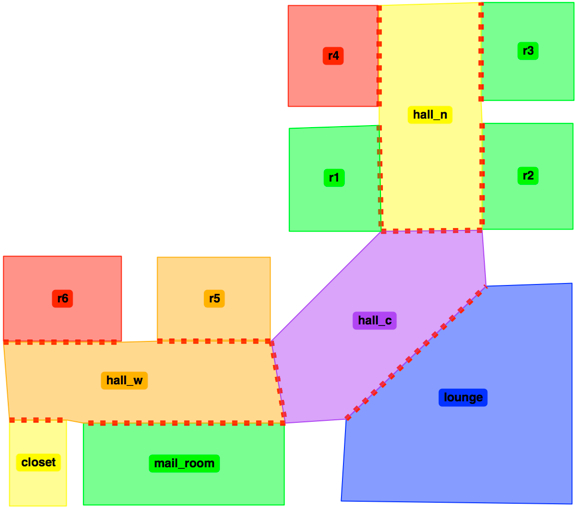
\includegraphics[width=0.99\columnwidth, clip]{./img/mailbotMap.jpg}
	\caption{\ldots} % TODO: Write stuff here
	\label{Fig:map}
\end{figure}

\ldots

% END
%
%\begin{myExample}\label{Ex:restaurant} Robotic Waiter \\
%	Overview of task \ldots
%\end{myExample}
%
%\begin{algorithm}
%	\textbf{Mission specification:} Robotic Waiter\\
%	{\small
%	\texttt{Group Customers is empty}\\
%	\texttt{Group Orders is empty}\\
%	\texttt{Group ... is empty}\\
%	\texttt{Group ... is empty}\\
%	
%	\texttt{Orders correspond to Customers}\\
%	\texttt{... correspond to...}\\
%	
%	\texttt{if you are activating any Orders then go to kitchen and do corresponding FoodPickUp and go to corresponding Customer and do corresponding ServeFood}\\
%	\texttt{...}\\
%	
%	\texttt{...}\\
%	}
%	
%	\textbf{Open World Settings:}\\
%	{\small
%	\texttt{if you are sensing newOrder then add to Orders}\\ % TODO: ... and add to corr. groups?
%	\texttt{...} 
%	}
%\end{algorithm}
%
%\begin{myExample}\label{Ex:planetxplore} Autonomous Planetary Exploration\\
%	Consider now the more futuristic scenario of autonomous planetary exploration using rovers. In order to lessen the dependency of the rover from the engineers on Earth, the rover will be given a mission specification that it should carry out autonomously. However, the need to redefine the mission will arise as the rover discovers interesting elements of its environment, such as new types of rock and regions interest. In these cases, the engineers and scientists on Earth should be able to extend the rover's mission specification without sacrificing correctness or rewriting the specification from scratch.
%	
%	Specifics: exploration, new stuff sensor, new requests.
%\end{myExample}
%
%\begin{algorithm}
%	\textbf{Mission specification:} Autonomous Planetary Exploration\\
%	{\small
%	\texttt{Group InterestingRegions is empty}\\
%	\texttt{Group PendingRequests is empty}\\
%	\texttt{Group Sites is empty}\\
%	\texttt{Group Actions is empty}\\
%	
%	\texttt{Sites correspond to Requests}\\
%	\texttt{Actions correspond to Requests}\\
%	
%	\texttt{Recharging is set on BatteryLow and reset on BatteryFull}\\
%	\texttt{if you are activating Recharging then stay there}\\
%	\texttt{infinitely often BatteryFull}\\
%	
%	\texttt{visit each InterestingRegion and do Panorama}\\
%	\texttt{if you are activating any PendingRequests then go to the corresponding Site and do the corresponding Action}\\
%	\texttt{each PendingRequest is toggled on the corresponding Site and the corresponding Action}\\
%	}
%	
%	\textbf{Exploration Settings:}\\
%	{\small
%	\texttt{do exploreMODE if and only if you are not activating Recharging}\\
%	\texttt{if you are sensing newInterestingRegion then add to InterestingRegions}\\
%	\texttt{...} 
%	}
%\end{algorithm}
%
%\begin{figure}[h]
%	\centering
%	\includegraphics[width=0.7\columnwidth, clip]{./img/planetXplore_regions.pdf}
%	\caption{Workspace for the autonomous planetary exploration scenario (to be updated and broken down to intermediate exploration steps).}
%	% TODO: Update this map. Regions should be around the land site! No mountain next to it either.
%	% Instead of the final map, show intermediate steps as the workspace is expanded.
%	\label{Fig:planetxplore}
%\end{figure}